
%--------------------------------------------------------------------
%--------------------------------------------------------------------
% Formato para los talleres del curso de Herramientas Computacionales
% Universidad de los Andes
% 2015-10
%--------------------------------------------------------------------
%--------------------------------------------------------------------

\documentclass[11pt,letterpaper]{exam}
\usepackage[utf8]{inputenc}
\usepackage[spanish]{babel}
\usepackage{graphicx}
%\usepackage{mdframed}
%\usepackage{tabularx}
\usepackage[absolute]{textpos} % Para poner una imagen completa en la portada
%\usepackage{multirow}
%\mdfdefinestyle{mystyle}{leftmargin=1cm,rightmargin=1cm,linecolor=red}
%\usepackage{float}
\usepackage{xcolor}
\usepackage{hyperref}
\hypersetup{colorlinks=false,linkbordercolor=red,linkcolor=green,pdfborderstyle={/S/U/W 1}}
\decimalpoint


\newcommand{\base}[1]{\underline{\hspace{#1}}}
\boxedpoints
\pointname{ pt}
%\extrawidth{0.75in}
%\extrafootheight{-0.5in}
\extraheadheight{-0.15in}
%\pagestyle{head}

%\noprintanswers
%\printanswers
\renewcommand{\solutiontitle}{}
\SolutionEmphasis{\color{blue}}

\usepackage{upquote,textcomp}
\newcommand\upquote[1]{\textquotesingle#1\textquotesingle} % To fix straight quotes in verbatim

\begin{document}
\begin{center}
{\Large Herramientas Computacionales} \\
Taller 9 - \textsc{Histogramas y Herramientas estadísticas}:\\

Fecha de publicación: {\small \it Abril de 2015}\\
\end{center}

\begin{textblock*}{40mm}(10mm,20mm)
  
\includegraphics[width=3cm]{logoUniandes.png}
\end{textblock*}

\begin{textblock*}{40mm}(161mm,20mm)
  
\includegraphics[width=3cm]{logoUniandes.png}
\end{textblock*}

\vspace{0.5cm}

\noindent El código que de solución a este taller debe ser entregado en un solo archivo con nombre:\\
 \verb+ApellidoEstudiante.py o .ipynb+ a través de \textbf{Sicuaplus}. El código debe llevar comentarios suficientes.

\vspace{0.5cm}

\begin{questions}

\question[50] {\bf Giro de Italia}

En el archivo \verb+giro_2014.csv+ se encuentran los tiempos totales de todos los corredores al terminar cada una de las 21 etapas del {\it Giro de Italia} del 2014. 

\begin{parts}

\part[25] Haga los histogramas para los tiempo acumulados de todos los corredores al terminar las etapas 2 y 21. Cuidado con los corredores retirados.

\begin{center}
	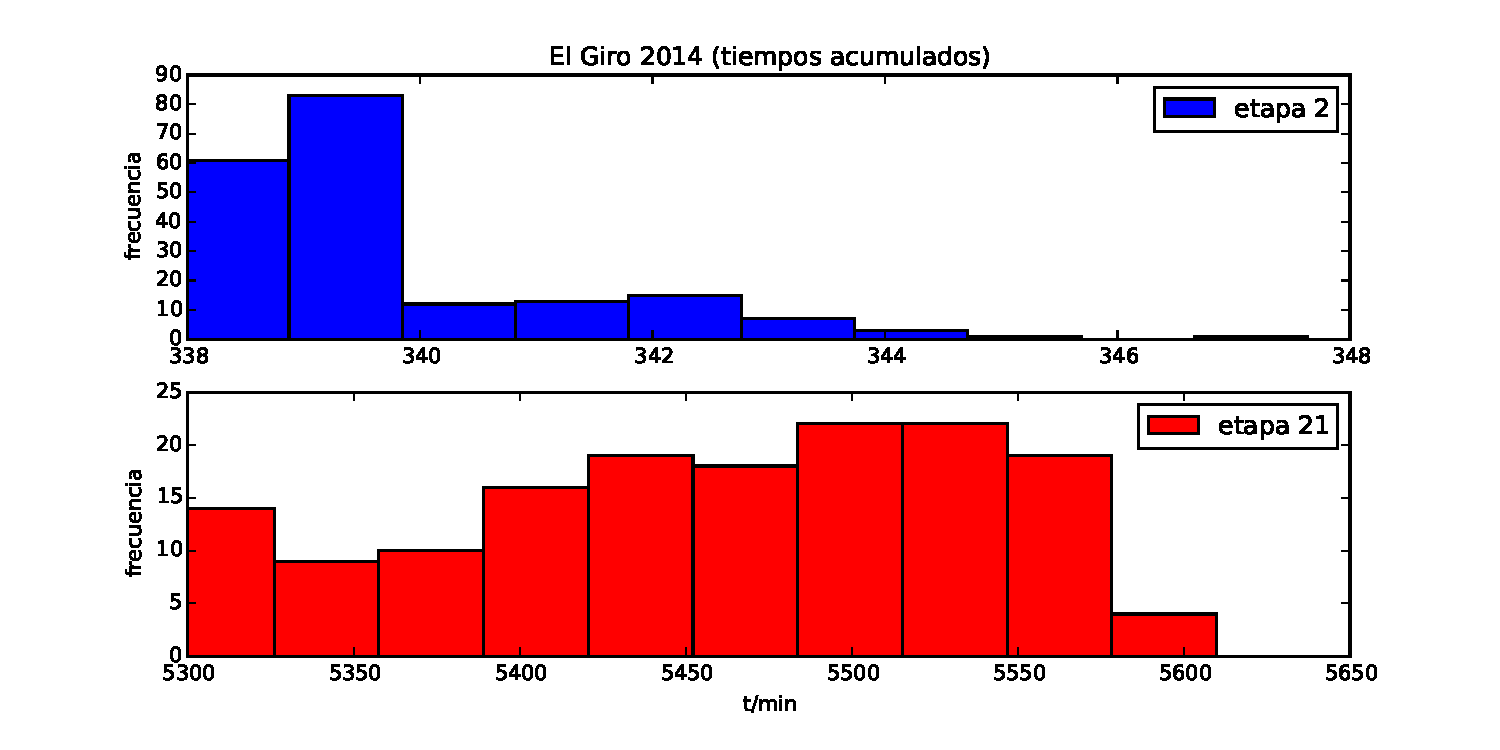
\includegraphics[width=0.85\textwidth]{./elgirodist.pdf}
\end{center}

\part[25] Guarde en un array los tiempos de cada etapa individual para los corredores que hicieron todas las etapas, y calcule la diferencia del tiempo de cada corredor con el ganador de cada etapa dividida por el tiempo ganador. Haga un histograma de todos estos tiempos relativos eligiendo opciones tales que el resultado sea similar al mostrado abajo.

\begin{center}
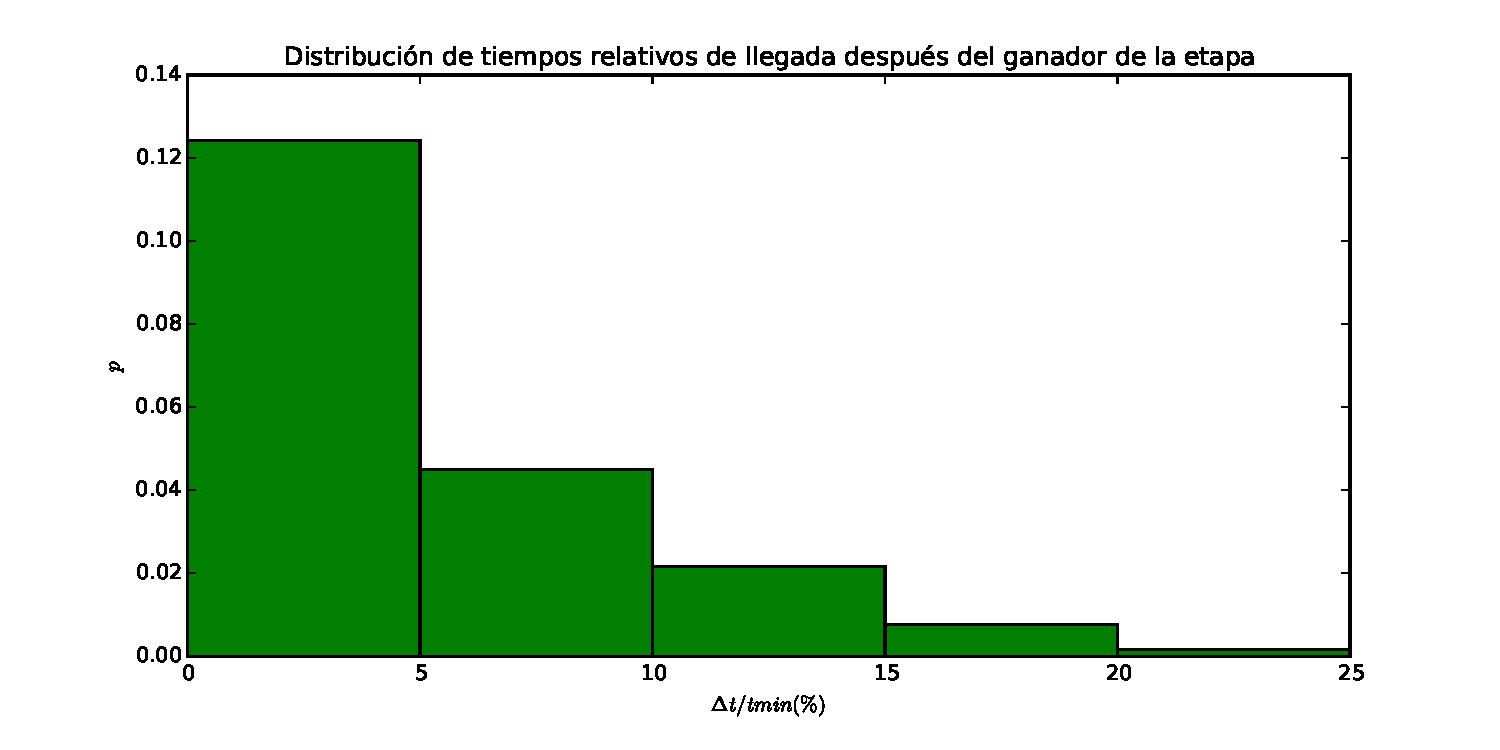
\includegraphics[width=0.7\textwidth]{tiempostodogiro.pdf}
\end{center}

\end{parts} 

\question[50]{\bf Doble distribución normal}

Imagine una distribución hipotética que utilice con igual probabilidad dos distribuciones normales. En concreto considerar la una centrada en $x=10$ y la otra en $x=20$ ambas con $\sigma=2$. 

\begin{parts}

\part[15] Genere 10000 números de dicha distribución usando la función \verb+random.normal+. Haga una histograma de esta distribución usando $25$ \verb+bins+. Normalice de tal manera qué el área del histograma sea 1.

\begin{center}
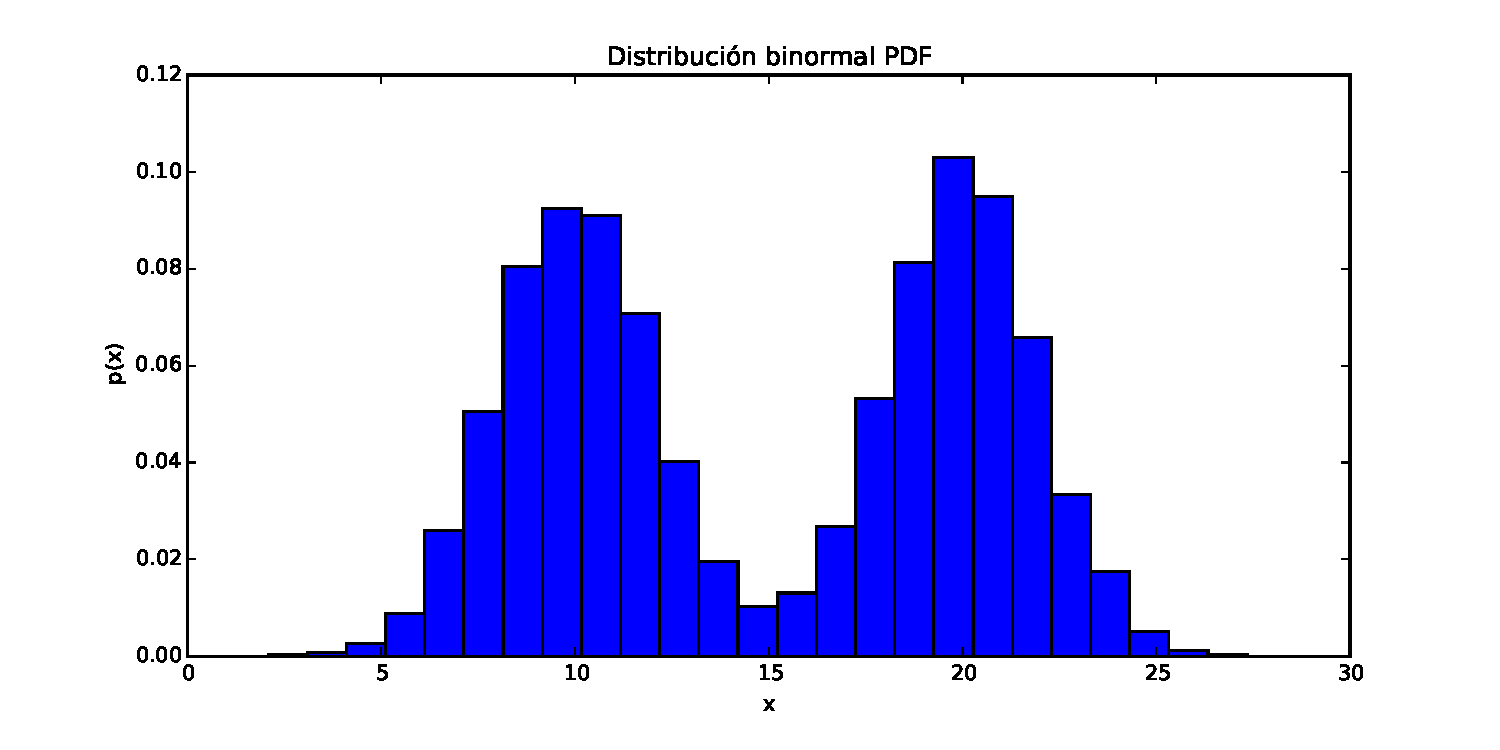
\includegraphics[width=0.7\textwidth]{binormalPDF.pdf}
\end{center}

\part[5] Grafique el histograma cumulativo de esta distribución.

\begin{center}
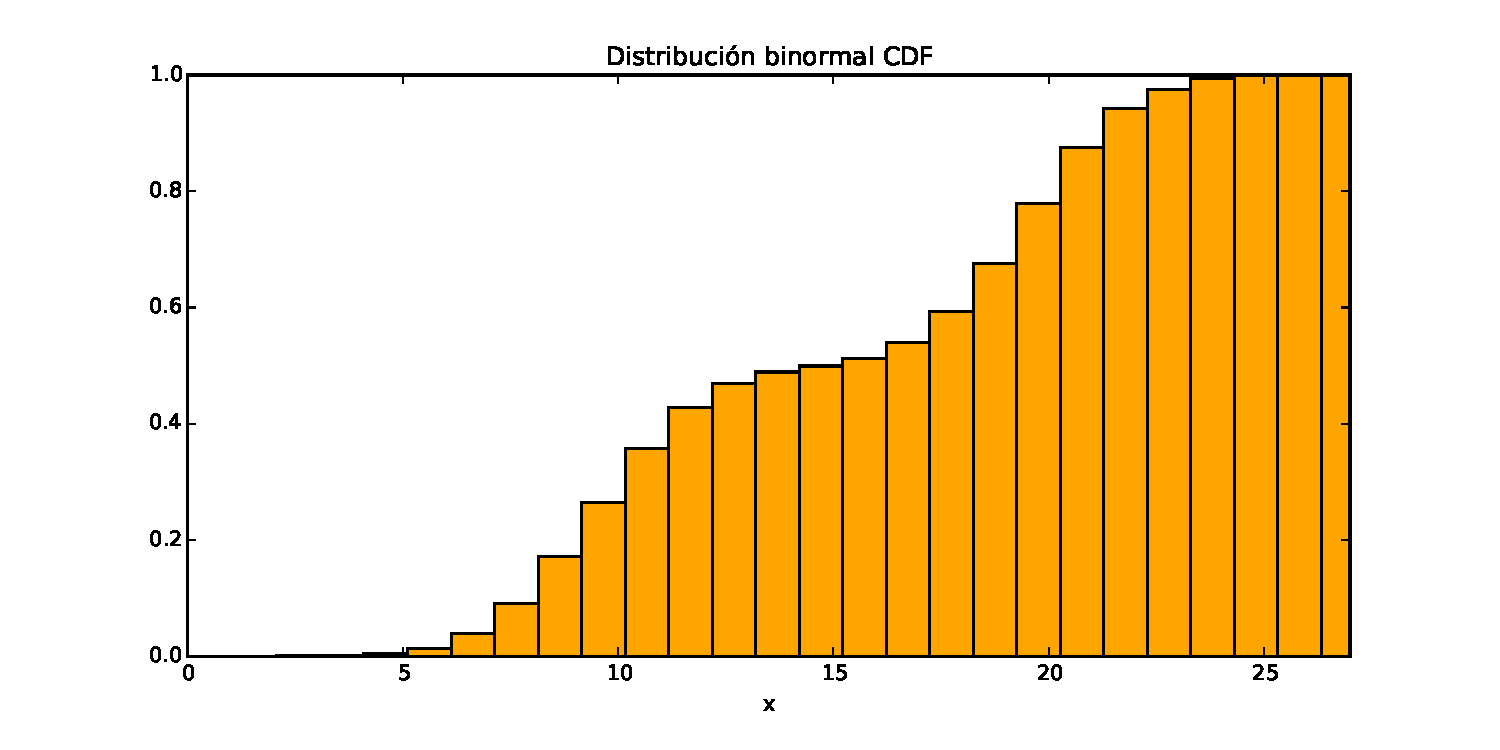
\includegraphics[width=0.7\textwidth]{binormalCDF.pdf}
\end{center}

\part[30] Escriba una función que genere números cuya probabilidad de salir este dada por dicha distribución usando los datos obtenidos en el primer literal. Esta función se debe llamar \verb+random_2normal+ y debe recibir por par\'ametro la cantidad de n\'umeros a generar. En ella implemente el método  \href{http://en.wikipedia.org/wiki/Inverse\_transform\_sampling}{Inverse Transform Sampling}. Puede ser de utilidad la función \verb+interp1d+ de \verb+scipy.interpolate+.

\end{parts}

\end{questions}




\end{document}
